\documentclass[10pt]{article}
\usepackage{report}
\usepackage[acronym]{glossaries}
\usepackage{rotating}
\usepackage{float}
\usepackage{siunitx}
\usepackage{array}
\usepackage[justification=centering]{caption}
\usepackage{booktabs}
\usepackage[usenames,dvipsnames,svgnames,table]{xcolor}
\usepackage[dvipsnames]{xcolor}
\usepackage{chngcntr}
\usepackage[utf8]{inputenc}
\usepackage{amssymb}
\usepackage{graphicx}
\usepackage{xspace}
\usepackage{subcaption}
\captionsetup{compatibility=false}

\newcommand{\mynote}[3]{
   \fbox{\bfseries\sffamily\scriptsize#1}
   {\small$\blacktriangleright$\textsf{\emph{\color{#3}{#2}}}$\blacktriangleleft$}}
\newcommand{\fp}[1]{\mynote{Fernando}{#1}{Red}}
\newcommand{\lle}[1]{\mynote{Long}{#1}{Cerulean}}

\newcommand{\ssmr}{\mbox{S-SMR}\xspace}
\newcommand{\ssmrshort}{Scalable SMR}
\newcommand{\ssmrlong}{Scalable State Machine Replication}
%
% DS-SRM
\newcommand{\dssmr}{\mbox{DS-SMR}}
\newcommand{\dssmrshort}{Dynamic S-SMR}
\newcommand{\dssmrlong}{Dynamic Scalable State Machine Replication}

\newcommand{\dynastar}{\mbox{DynaStar}\xspace}


\title{Bridge Proof of Concept}
\author{Long Hoang Le}
\date{\today}

\rfoot{\small{Proof of Concept project description $|$ \thepage}}
\lfoot{
\includegraphics[width=0.5in]{logo.png}}


\begin{document}
% \pagenumbering{roman} % roman page numbers

\addcontentsline{toc}{section}{TITLE PAGE}
\thispagestyle{empty} % This will hide pagenumber in title page


% Title page (Design in your own way)

{
	\thispagestyle{empty}
	\centering
	\normalsize
	  
	
\includegraphics[width=1.3in]{logo.png}\\[1cm]
	% \includegraphics[height=1.6in]{fig/tu-logo}\\
	{\large{\bf Proof of Concept}}\\
	Project description\\[4.5cm]
	
	Long Hoang Le \\
	\large{\bf Scaling blockchain: optimized partitioning as a service}\\[1.5cm]
	
}

%!TEX root =  main.tex
\newpage
\section{Summary}
Since Bitcoin's initial launch in 2009, blockchain technologies have attracted
extensive worldwide attention. Since then, several blockchain implementations
were proposed, each focusing on solving specific shortcomings of the original
blockchain proposal. Some implementations focus on special features, such as
smart contract support \cite{buterin2013ethereum, elrom2019neo}, privacy
\cite{alonso2018monero}. Some others allow enterprises to create private
blockchains, where only a defined set of entities can participate
\cite{androulaki2018hyperledger}. The growing adoption of blockchain-based
systems has raised many new challenges. In particular, two primary and urgent
challenges in this context are scalability and interoperability. Scalability is
the ability to achieve a target throughput and latency in the presence of
increasing workload without compromising the decentralized nature of
blockchains. Interoperability allows communication and data exchanging between
multiple different blockchains. 

Scalable performance could be achieve by state partitioning (e.g.,
\cite{facebookTAO, sciascia2012sdur, aguilera2007sinfonia}). State partitioning
is challenging, however, due to fundamental differences between previous domains
and blockchain, notably the failure model. With its decentralized nature, there
is no single entity in a blockchain system that contains information of all
objects in the network, which makes it difficult for blockchain clients to
locate objects in the presence of partitioning. In addition, with the lacking of
overall information, choosing a partition to place the objects in order to
maximize the balance between partitions is not effective. Even if enough
information is available, finding a good partitioning is a complex optimization
problem~\cite{curino2010sch,taft2014est}. Interoperability, on the other hand,
is gaining more attention in the blockchain community. Some blockchain systems
has introduced inter blockchain communication (IBC) protocols that enable
communication and data exchanging between multiple blockchains, allows users to
choose where to place smart contracts \cite{kwon2016cosmos, thomas2015protocol,
kokoris2018omniledger, al2017chainspace}. Moreover, some solutions start to
appear that allow smart contracts to move between blockchains
\cite{fynn2020move, back2014enabling, herlihy2018atomic}.

Scalability and interoperability are different problems of blockchain, they are
however in need a common component: an oracle that provides some information of
the blockchains. A partitioned blockchains needs an overview of the partitioning
in order to place the objects and contract on an optimized location to maintain
the balance of the network and therefore increase the performance. For
blockchains to interact with each other, some information of the other
blockchains like the cost of transaction, the performance of the network is also
necessary. This project proposes an oracle service that provides such
information. The oracle service consists of two main components, one on-chain
and one off-chain. The on-chain component is in the form of a smart contract,
replies to the request of user smart contract. The off-chain component is a
service that monitors the blockchains by analyzing the transaction history.
After receiving a request from user smart contract, the on-chain and off-chain
components communicate to extract the necessary information for the request.
User smart contract pays per-query fees to get the hints from the oracle
service. The cost of each query depends on the amount of information returned.
With the information provided by the oracle, the blockchain system can
effectively choose a partition to place objects to maximize the balance of the
network, thus increase the transaction speed, as well as optimizing the the
execution cost with cross-chain transaction.

% In addition, unlike some other scaling proposals that require
% extensive modification of the current blockchain code, our proposal will work
% with most of the blockchains that support smart contract, without changing
% client code.


% fee changes base on the hints
\newpage
\section{Project description}

\subsection{Research background}

In the core of most blockchains, assets are transferred
under the control of custom scripts that enforce necessary conditions to
transfer an asset from one party to another. The custom script (so-called
\emph{smart contracts}) is a self-executable, self-enforceable and
self-verifiable published on the blockchain. Being the first generation of
blockchain, Bitcoin has very limited support for smart contract. On the other
hand, later generations of blockchain (Etherum, NEO, Stellar, etc.) address this
problem by providing a general purpose programmable infrastructure (as known as
smart contract), where the blockchain does not only store financial data but
also have the capability of deploying and executing custom code on the
blockchain system. This increases the flexibility of the system and enable more
options for optimization.

% Ethereum is after Bitcoin the second-largest cryptocurrency platform by market
% capitalization. Unlike Bitcoin, Ethereum supports programmable smart contracts
% with an entire programming language along with it, running in Ethereum Virtual
% Machine (EVM) \cite{ethereum:evm}. The flexibility within a smart contract
% enables users to implement their own autonomous execution logic on blockchains
% \cite{delmolino2016step, buterin2014next, kosba2016hawk}.


\subsubsection{Blockchain and scalability problem}
While the demand for blockchain solutions is increasing over years since the
first introduction of Bitcoin, the performance of mainstream blockchains is
still a barrier to the adoption of blockchain technology. As a global payment
system, Visa is capable of processing around 24,000 transactions per second on
average \cite{visa}, while the number is 7 and 15 for Bitcoin and Etherum
respectively \cite{ethereum:sharding, nakamoto2019bitcoin}. Scaling the
performance of blockchain systems has become a hot topic for both industry and
academia, with many proposals. Those proposals varies from optimizing the
performance of the consensus protocols \cite{dang2019towards}, partitioning the
blockchain \cite{wang2019sok} to shifting the computation from the blockchain
(on-chain) to the outside (off-chain) \cite{teutsch2019scalable,
network2018cheap}. Being the first generation of blockchain, Bitcoin has very
limited support for programmable transactions, thus also has limited options for
scaling that doesn't require changes in its protocol. On the other hand, later
generations of blockchain (Etherum, NEO, Stellar, etc.) address this problem by
providing a general purpose programmable infrastructure (as known as smart
contract), where the blockchain does not only store financial data but also have
the capability of deploying and executing custom code on the blockchain system.
This increases the flexibility of the system and enable more options for
optimization.

\subsubsection{Scaling by partitioning}
Among all proposed method for scaling the performance, sharding the blockchain
state is an effective and practical solution, as it can overcome both
performance and scalability problems of blockchain. Partitioning (or
\emph{sharding}) is a technique that divides the state of a service or a system
in multiple partitions so that most requests or transactions access one
partition only and are equally distributed among partitions. As a result,
partitions can work in parallel to maximize the performance and improve the
throughput. On the downside of this approach, if a transaction accesses data
from multiple partitions, those partitions have to coordinate to execute the
transaction, thus increase the cost of the execution. The major challenge in
this approach is to come up with an optimized partitioning scheme to minimize
the number of cross-partition transactions, and also an effective execution
scheme that could handle multi-partition transactions.

\subsubsection{State machine replication (SMR) and Scaling SMR}
State machine replication, also called active replication, is a common approach
to building fault-tolerant systems \cite{Lam78, Sch90}. Participants in a
replicated state machine system form agreement on a sequence of transactions and
apply them in sequence order deterministically to the reach the same state. With
its simple yet effective execution model, state machine replication is at the
core of many blockchain systems \cite{baudet2019state, cachin2016architecture}.
In terms of scalability, unfortunately, classic state machine replication does
not scale. Increasing the number of replicas will not scale performance since
each replica must execute every command. In the work called Dynamic scalable
state machine replication (\dssmr), Le \emph{et al.} proposed an approach for
scaling the performance of SMR by allowing SMR system to reconfigure its data
placement on-the-fly. By moving data ``on demand'' to maximize the number of
single partition requests, \dssmr{} allows SMR system to adapt the partitioning
scheme as workloads change. To keep track the partition of objects in the
system, \dssmr{} maintain a location oracle with a global view of the
application state. The result of this work shows that scalable performance could
be achieved in a replication system with a good partitioning scheme. In a later
work, the authors introduced \dynastar, an optimized partitioning solutions for
SMR. \dynastar shows that by using the data of the location oracle to come up
with an optimized partitioning, scalable performance is achievable for
real-world application. The authors also presented a detailed experimental
evaluation of \dynastar using the TPC-C benchmark and a social network service
populated with a real social network graph. Figure \ref{fig:tpcc} shows the
performance evaluation of \dynastar with TPC-C benchmark. Figure
\ref{fig:tpcc}(a) depicts the impact of partitioning on the performance of a
system before and after an optimized partitioning configuration is applied.
Figure \ref{fig:tpcc}(b) shows the scalability of \dynastar when increase the
size of the system (adding more data and computational resources). It's worth to
note that in a TPC-C benchmark, the average rate of mutli-partition transactions
is 15\%.

\begin{figure*}[ht!]
  \centering
  \begin{subfigure}{.48\textwidth}
    \centering
    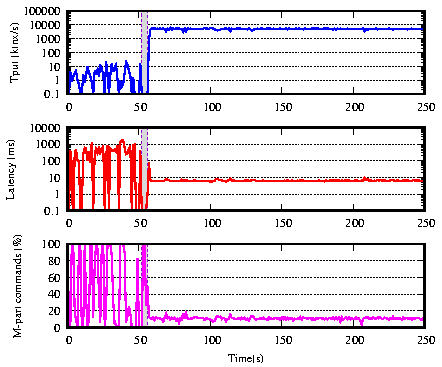
\includegraphics[width=0.8\columnwidth]{figures/tpcc-detail-dynastar}
  \caption{Repartitioning in \dynastar; throughput (top), objects exchanged
  between partitions (middle), and percentage of multi-partition commands
  (bottom).}
  \end{subfigure}
  \begin{subfigure}{.48\textwidth}
    \centering
    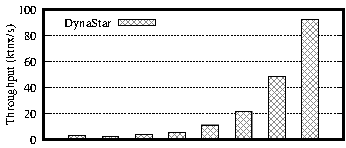
\includegraphics[width=\textwidth]{./figures/tpcc-scaling-tp-lat-bridge}
    \caption{Performance scalability with TPC-C. Throughput (in thousands of transactions per second, ktps)}
  \end{subfigure}
  \caption{Dynastar performance with TPC-C Benchmark}
  \label{fig:tpcc}
\end{figure*}

\subsection{Innovation potential and market review} 

\subsubsection{General ideas}

\subsubsection{General ideas}

\subsubsection{Integrability}
This proposal is based on an assumption that contracts and data can move across
blockchain. Moving and sharing data across blockchain systems or between
partitions in a blockchain (interoperability) has been in the blockchain
wishlist for some time. A protocol with this goals has been proposed in the
Ethereum research forum concurrently with the development of this work
\cite{buterin2018yanking}. In another work, a move primitive introduced by Fynn \emph{et al.}
\cite{fynn2020move} allows programmable blockchains to interoperate by moving
contracts and data from one to another. This solution is plugable as a smart
contract, requires no modification to the blockchain. 

With the on-chain component in the form of smart contract, our proposed system
could be integrated to existing blockchain systems easily without any change in
the blockchain protocol. 

\subsubsection{Expected outcome}

In an analysis in \cite{fynn2020move}, the author performed an extensive study
on the impact of partitioning Ethereum blockchain. The study showed that even on
a workload that was not created for a sharded system, the partitioning scheme
could achieve a rate of less then 10 percents of cross partition transaction. 


\subsection{Implementation strategy}

\subsection{Project plan}


\newpage
\phantomsection
\addcontentsline{toc}{section}{REFERENCES}

%dont write anything here
%dont write anything here

%visit http://scholar.google.com/ search and get BibTeX format and paste in biblio.bib file. It appears automatically in references whenever you cite it somewhere in your document.


%EXAMPLE OF BIBTEX citation from google scholars
% @book{latex2e,
%   author = {Leslie Lamport},
%   year = {1994},
%   title = {\LaTeX: a Document Preparation System},
%   publisher = {Addison Wesley},
%   address = {Massachusetts},
%   edition = {2}
% }


%CITE LIKE THIS IN YOUR LATEX DOCUMENT
% \cite{latex2e}


\bibliographystyle{IEEEtran}
\bibliography{references}





\end{document}
